\subsection{Caso d'uso UC1: Creazione nuova presentazione}
\begin{figure}[h] 
	\centering 
	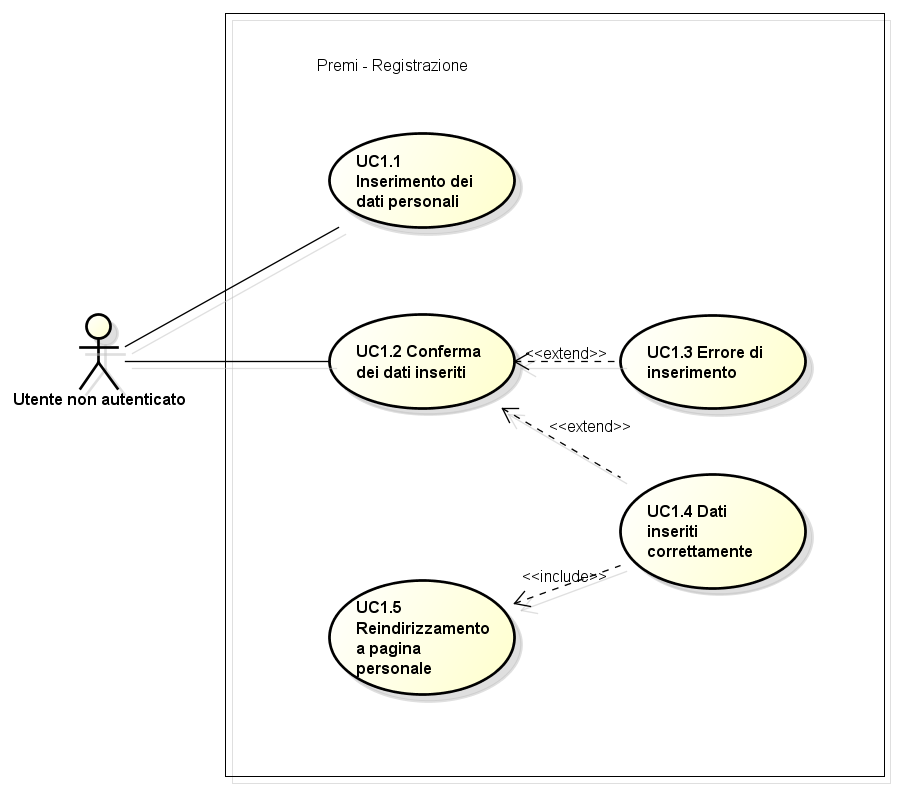
\includegraphics[scale=0.45] {img/UC1.png} 
	\caption{UC1 - Creazione nuova presentazione} 
\end{figure}

\begin{itemize}
	\item \textbf{Attori:} Utente;
	\item \textbf{Scopo e descrizione:} L'utente sta creando una nuova presentazione di slide. Per completare l'operazione deve inserire almeno una slide vuota. Potrà anche inserire una o più: immagine, casella di testo, dato \gls{real time}. Potrà essere scelto anche l'effetto di transizione da una slide ad un'altra;
	\item \textbf{Precondizione:} Il sistema mostra la schermata di creazione di una presentazione e l'utente vuole creare una nuova slide;
	\item \textbf{Flusso degli eventi:}
	\begin{enumerate}
		\item L'utente crea una nuova slide [UC1.1];
		\item L'utente può inserire un'immagine o più [UC1.2];
		\item L'utente carica un file per inserire l'immagine [UC1.6];
		\item L'utente può inserire una casella di testo o più [UC1.3];
		\item L'utente sceglie la formattazione del testo [UC1.7];
		\item L'utente può inserire dei dati \gls{real time} [UC1.4];
		\item L'utente può scegliere un effetto di transizione [UC1.5];
	\end{enumerate}
	\item \textbf{Postcondizione:} Il sistema mostra le operazioni effettuate dall'utente.
\end{itemize}

\subsection{Caso d'uso UC1.1: Inserire nuova slide}
\begin{itemize}
	\item \textbf{Attori:} Utente;
	\item \textbf{Scopo e descrizione:} L'utente crea una nuova slide nella presentazione per poter inserire del contenuto;
	\item \textbf{Precondizione:} Il sistema è in attesa che l'utente crei una nuova slide;
	\item \textbf{Postcondizione:} Il sistema ha creato la nuova slide.
\end{itemize}

\subsection{Caso d'uso UC1.2: Inserire un'immagine}
\begin{itemize}
\item \textbf{Attori:} Utente;
\item \textbf{Scopo e descrizione:} L'utente deve inserire l'immagine da mettere nella slide;
\item \textbf{Precondizione:} Il sistema è in attesa che l'utente selezioni l'immagine;
\item \textbf{Postcondizione:} Il sistema ha caricato l'immagine selezionata dall'utente.
\end{itemize}

\subsection{Caso d'uso UC1.3: Inserire casella di testo}
\begin{itemize}
\item \textbf{Attori:} Utente;
\item \textbf{Scopo e descrizione:} L'utente deve inserire una casella di testo nella slide;
\item \textbf{Precondizione:} Il sistema è in attesa che l'utente crei una casella di testo;
\item \textbf{Postcondizione:} Il sistema ha creato la casella di testo.
\end{itemize}

\subsection{Caso d'uso UC1.4: Inserire dati real time}
\begin{itemize}
	\item \textbf{Attori:} Utente;
	\item \textbf{Scopo e descrizione:} L'utente deve inserire dei dati \gls{real time};
	\item \textbf{Precondizione:} Il sistema è in attesa che l'utente inserisca i dati \gls{real time};
	\item \textbf{Postcondizione:} Il sistema ha inserito i dati \gls{real time}.
\end{itemize}

\subsection{Caso d'uso UC1.5: Scegliere effetto di transizione}
\begin{itemize}
	\item \textbf{Attori:} Utente;
	\item \textbf{Scopo e descrizione:} L'utente deve scegliere l'effetto di transizione da dare alla slide;
	\item \textbf{Precondizione:} Il sistema è in attesa che l'utente selezioni l'effetto desiderato;
	\item \textbf{Postcondizione:} Il sistema ha inserito l'effetto di transizione.
\end{itemize}

\subsection{Caso d'uso UC1.6: Caricare file}
\begin{figure}[h] 
	\centering 
	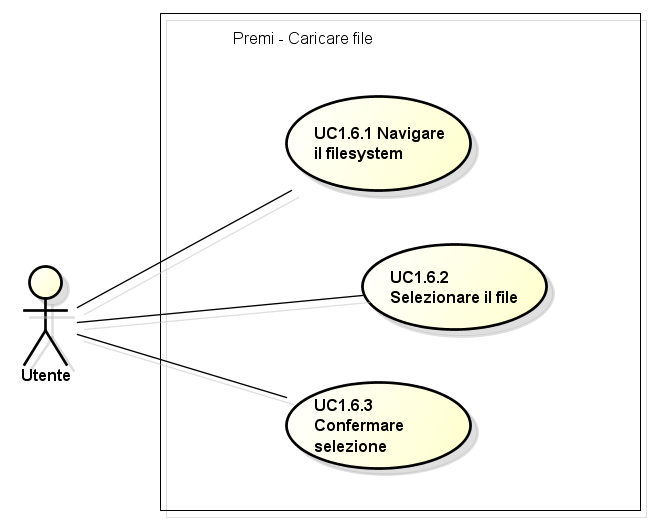
\includegraphics[scale=0.45] {img/UC1.6.png} 
	\caption{UC1.6 - Caricare file} 
\end{figure}

\begin{itemize}
	\item \textbf{Attori:} Utente;
	\item \textbf{Scopo e descrizione:} L'utente deve caricare un file. Naviga il \gls{filesystem} cercando il file desiderato, lo seleziona e conferma la selezione caricando il file;
	\item \textbf{Precondizione:} Il sistema è in attesa che l'utente selezioni il file;
	\item \textbf{Flusso degli eventi:}
	\begin{enumerate}
		\item L'utente naviga il \gls{filesystem} alla ricerca del file desiderato [UC1.6.1];
		\item L'utente seleziona il file [UC1.6.2];
		\item L'utente conferma il file selezionato [UC1.6.3].
	\end{enumerate}
	\item \textbf{Postcondizione:} Il sistema ha caricato il file selezionato dall'utente e lo ha inserito nella slide.
\end{itemize}

\subsection{Caso d'uso UC1.6.1: Navigare il filesystem}
\begin{itemize}
	\item \textbf{Attori:} Utente;
	\item \textbf{Scopo e descrizione:} L'utente può navigare il \gls{filesystem} per selezionare la cartella dentro la quale è contenuto il file desiderato;
	\item \textbf{Precondizione:} Il sistema è in attesa che l'utente selezioni una cartella;
	\item \textbf{Postcondizione:} Il sistema ha aggiornato la cartella corrente con quella scelta dall'utente.
\end{itemize}

\subsection{Caso d'uso UC1.6.2: Selezionare il file}
\begin{itemize}
	\item \textbf{Attori:} Utente;
	\item \textbf{Scopo e descrizione:} L'utente deve selezionare il file che intende caricare;
	\item \textbf{Precondizione:} Il sistema mostra i file contenuti nella cartella precedentemente selezionata;
	\item \textbf{Postcondizione:} Il sistema evidenzia il file scelto dall'utente.
\end{itemize}

\subsection{Caso d'uso UC1.6.3: Confermare selezione}
\begin{itemize}
	\item \textbf{Attori:} Utente;
	\item \textbf{Scopo e descrizione:} L'utente conferma che il file selezionato in precedenza è quello corretto;
	\item \textbf{Precondizione:} Il sistema ha selezionato il file indicato dall'utente;
	\item \textbf{Postcondizione:} Il sistema ha caricato il file scelto precedentemente dall'utente.
\end{itemize}

\subsection{Caso d'uso UC1.7: Scegliere formattazione del testo}
\begin{figure}[h] 
	\centering 
	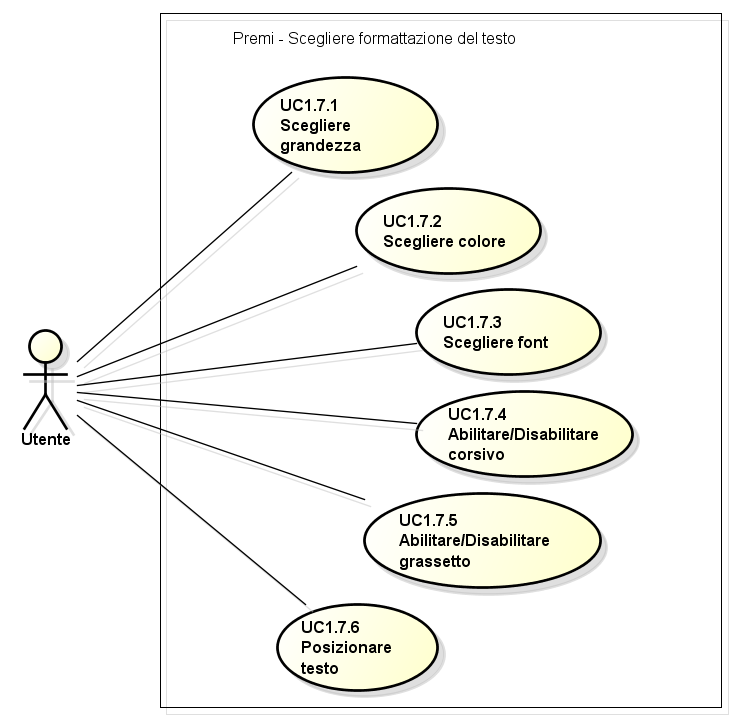
\includegraphics[scale=0.45] {img/UC1.7.png} 
	\caption{UC1.7 - Scegliere formattazione del testo} 
\end{figure}

\begin{itemize}
	\item \textbf{Attori:} Utente;
	\item \textbf{Scopo e descrizione:} L'utente può modificare l'aspetto del testo contenuto in una casella di testo. L'utente seleziona il testo e poi sceglie che modifiche effettuare;
	\item \textbf{Precondizione:} Il sistema è in attesa che l'utente selezioni la modifica da apportare al testo e il testo da modificare è selezionato;
	\item \textbf{Flusso degli eventi:}
	\begin{enumerate}
		\item L'utente può cambiare la grandezza del testo [UC1.7.1];
		\item L'utente può cambiare il colore del testo [UC1.7.2];
		\item L'utente può cambiare il \gls{font} del testo [UC1.7.3];
		\item L'utente può abilitare o disabilitare il testo in corsivo [UC1.7.4];
		\item L'utente può abilitare o disabilitare il testo in grassetto [UC1.7.5];
		\item L'utente può spostare il testo in una nuova posizione [UC1.7.6].
	\end{enumerate}
	\item \textbf{Postcondizione:} Il sistema ha apportato le modifiche scelte al testo.
\end{itemize}

\subsection{Caso d'uso UC1.7.1: Scegliere grandezza}
\begin{itemize}
	\item \textbf{Attori:} Utente;
	\item \textbf{Scopo e descrizione:} L'utente può cambiare la grandezza del testo;
	\item \textbf{Precondizione:} Il testo da modificare è selezionato;
	\item \textbf{Postcondizione:} Il testo è stato ingrandito o rimpicciolito secondo la scelta dell'utente.
\end{itemize}

\subsection{Caso d'uso UC1.7.2: Scegliere colore}
\begin{itemize}
	\item \textbf{Attori:} Utente;
	\item \textbf{Scopo e descrizione:} L'utente può cambiare il colore del testo;
	\item \textbf{Precondizione:} Il testo da modificare è selezionato;
	\item \textbf{Postcondizione:} Il testo è stato colorato secondo la scelta dell'utente.
\end{itemize}

\subsection{Caso d'uso UC1.7.3: Scegliere font}
\begin{itemize}
	\item \textbf{Attori:} Utente;
	\item \textbf{Scopo e descrizione:} L'utente può cambiare il \gls{font} del testo;
	\item \textbf{Precondizione:} Il testo da modificare è selezionato;
	\item \textbf{Postcondizione:} Il testo ha cambiato \gls{font} secondo la scelta dell'utente.
\end{itemize}

\subsection{Caso d'uso UC1.7.4: Abilitare/Disabilitare corsivo}
\begin{itemize}
	\item \textbf{Attori:} Utente;
	\item \textbf{Scopo e descrizione:} L'utente può abilitare o disabilitare la scrittura in corsivo;
	\item \textbf{Precondizione:} Il testo da modificare è selezionato oppure è stata selezionata la casella di testo nella quale poter scrivere;
	\item \textbf{Postcondizione:} Il testo è stato modificato secondo la scelta dell'utente.
\end{itemize}

\subsection{Caso d'uso UC1.7.5: Abilitare/Disabilitare grassetto}
\begin{itemize}
	\item \textbf{Attori:} Utente;
	\item \textbf{Scopo e descrizione:} L'utente può abilitare o disabilitare la scrittura in grassetto;
	\item \textbf{Precondizione:} Il testo da modificare è selezionato oppure è stata selezionata la casella di testo nella quale poter scrivere;
	\item \textbf{Postcondizione:} Il testo è stato modificato secondo la scelta dell'utente.
\end{itemize}

\subsection{Caso d'uso UC1.7.6: Posizionare testo}
\begin{itemize}
	\item \textbf{Attori:} Utente;
	\item \textbf{Scopo e descrizione:} L'utente può spostare una casella di testo in una nuova posizione;
	\item \textbf{Precondizione:} La casella di testo da spostare è stata selezionata;
	\item \textbf{Postcondizione:} La casella di testo è stata spostata secondo la scelta dell'utente.
\end{itemize}